\documentclass[11pt]{article}

\usepackage[margin=1in]{geometry}
\usepackage{amsmath}
\usepackage{booktabs}
\usepackage{graphicx}
\usepackage{siunitx}
\usepackage{subcaption}
\usepackage{float}
\usepackage[hidelinks]{hyperref}

\title{Building, Modeling, and Field Testing of an Electromagnetic Seismometer}
\author{Zhicheng Gong, Jianing Pan}
\date{April 6, 2026}

\begin{document}

\maketitle

\begin{abstract}
We built and tested a slinky based seismometer that converted vertical motion into an electrical signal by electromagnetic induction. After adding an op-amp stage and Arduino-jAmaSeis readout, we tested the instrument on a campus bridge and near a bus loop. The bridge experiment produced clear signals from running and jumping, while the bus loop measurement was harder to interpret because multiple environmental sources contributed to the recorded waveform. We also calculated a theoretical sensitivity curve and compared it with FFTs of the measured data. This showed that the default digital acquisition chain strongly shapes the recorded spectrum, while the bridge post-event ringing still reveals the mechanical resonance of the spring-mass system. Overall, the instrument worked well as a low frequency vibration detector, but source identification in real world data remained limited.
\end{abstract}

\section{Introduction}
In this project we constructed a compact seismometer that used a suspended magnet and a surrounding coil inside a vertical tube. When the base of the instrument moved, the magnet and slinky did not follow the motion instantaneously, so the coil and magnet moved relative to one another. By Faraday's law of electromagnetic induction, that relative motion induced a voltage in the coil. The induced signal was small, so the complete instrument also required an amplifier and a digital recording stage.

Besides from building and testing the instrument, we focused on two types of measurements. First, we carried out controlled bridge tests in which one group member generated vibrations by walking and jumping at a known location. Second, we performed a field measurement near the campus bus loop, where the source was less controlled and the coupling between the source and the instrument was expected to be weaker. We also calculated the theoretical sensitivity of the seismometer from a simple model of the harmonic oscillator and the Arduino based acquisition chain in order to predict the instrument response and to understand whether the observed frequency content was affected by the physics of the seismometer itself or by the subsequent electronic and digital processing.

\section{Method}
The mechanical seismometer consisted of a spring, a suspended magnet, and a coil housed inside a cylindrical tube. A 3D printed support held the slinky at the top of the tube. Before each measurement session we followed the calibration procedure described in the seismometer manual. The three set screws on the base were adjusted until the slinky hung centrally within the damping tube. The magnet height was then adjusted until a magnet could be seen in the gap of the coil housing at equilibrium. This levelling step was repeated whenever the instrument was moved because even a small tilt changed the resting position and reduced the quality of the data.

After levelling, we connected the coil directly to an oscilloscope to verify that the instrument responded to disturbances. Tapping the table or disturbing the apparatus by hand produced visible low-frequency variations in the waveform, confirming that the coil output changed when the magnet moved relative to the tube.

An amplification stage shown in Figure \ref{fig:circuit} is then connected. The circuit used a single \SI{5}{\volt} supply and a midpoint bias of \SI{2.5}{\volt} produced by a \SI{10}{\kilo\ohm}-\SI{10}{\kilo\ohm} divider. The bias node was bypassed to ground with both \SI{1}{\micro\farad} and \SI{0.01}{\micro\farad} capacitors so that it acted as a comparatively quiet virtual reference over a wide range of frequencies. The op-amp was then used in an inverting-feedback configuration: the non-inverting input was held at \SI{2.5}{\volt}, the coil was connected to the inverting input, and the feedback path from output to inverting input consisted of an \SI{866}{\kilo\ohm} resistor in parallel with a \SI{330}{\pico\farad} capacitor. The oscilloscope was used again with AC coupling on both channels to compare the coil signal with the amplified output and to remove the \SI{2.5}{\volt} DC bias from the display. Once the gain stage was working, the output was connected to analog pin A0 of the Arduino and the provided \texttt{nerdaqII} code was uploaded. The real time data stream was then monitored in jAmaSeis.

\begin{figure}[ht]
  \centering
  \begin{subfigure}[t]{0.6\linewidth}
    \centering
    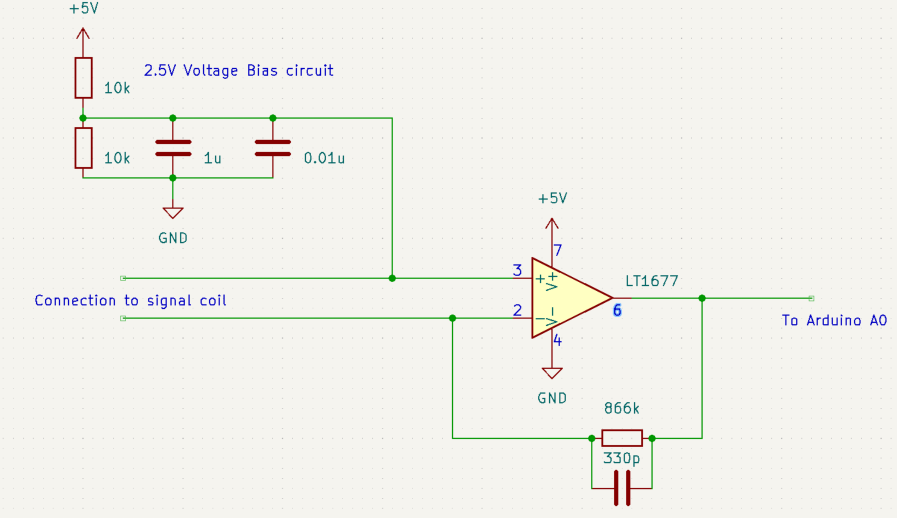
\includegraphics[width=\linewidth]{images/manual_figure6.png}
    \caption{Circuit diagram from the manual.}
  \end{subfigure}
  
  \vspace{0.8em}
  
  \begin{subfigure}[t]{0.6\linewidth}
    \centering
    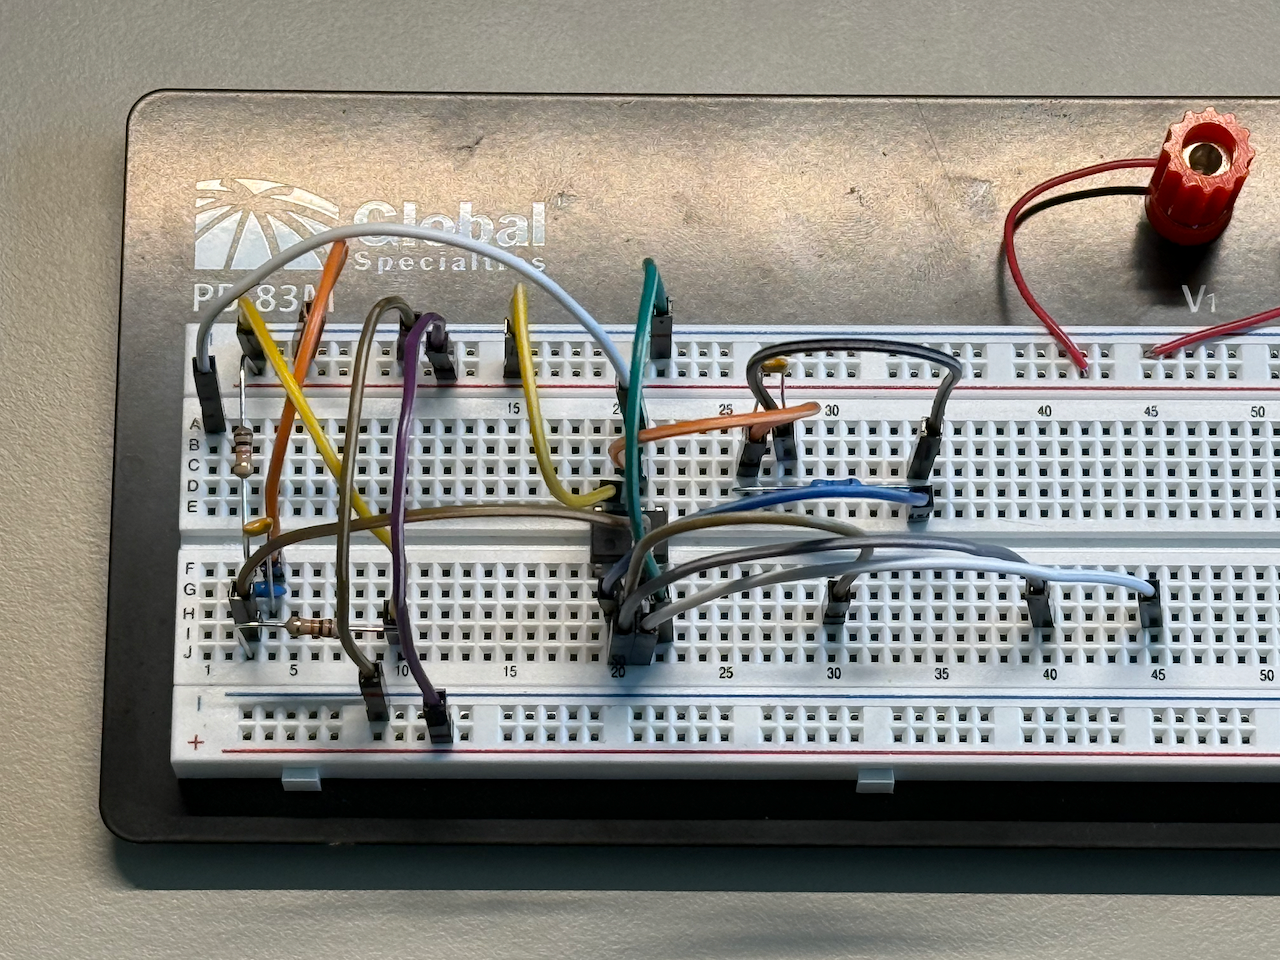
\includegraphics[width=\linewidth]{images/breadboard.png}
    \caption{Breadboard implementation used in the experiment.}
  \end{subfigure}
  \caption{Amplifier circuit used for the seismometer.}
  \label{fig:circuit}
\end{figure}

For the controlled sensitivity test, we moved the instrument to the bridge between the science buildings, levelled it again, and placed the instrument at the midpoint of the bridge. We then recorded data while one group member walked, ran, and jumped at different distances from the seismometer. One person watched the jAmaSeis display while the other generated the disturbance, which made it possible to identify the response windows more confidently.

For the real world measurement, we placed the seismometer near the campus bus loop and recorded data while buses passed. In a 15 minutes window, we recorded the output and nearby events. In this setting the source was not under our control, so the exact time and strength of each vibration were less certain than in the bridge test.

\section{Theory}
We can numerically calculate the sensitivity of the equipment by combining the frequency response of the three stages of the seismometer: a mechanical oscillator, an analog amplifier, and a digital acquisition and filtering stage. 

Mechanically, the spring and suspended magnet behave like a damped, base excited harmonic oscillator. We observed that the mass oscillated about 50 times in 60 seconds, which gives a natural frequency of about
\[
f_n \approx \frac{50}{60} \approx \SI{0.83}{\hertz}.
\]
For this relative sensitivity model, we assume that the input vibration is a sinusoidal wave with fixed displacement amplitude $Y$ at each frequency. Then the relative displacement amplitude $Z$ between the magnet and the coil is
\[
\left| \frac{Z}{Y} \right|
= \frac{r^2}{\sqrt{(1-r^2)^2 + (2 \zeta r)^2}},
\qquad
r = \frac{f}{f_n}.
\]
Because the induced voltage is proportional to relative velocity rather than relative displacement, the mechanical contribution to sensitivity scales like
\[
|H_{\text{mech}}(f)| \propto 2 \pi f \left| \frac{Z}{Y} \right|.
\]
This means the response is small at very low frequency, becomes largest near resonance, and then must still be interpreted together with the analog and digital filters before deciding which disturbances the instrument records most strongly.

The analog amplifier shapes the response before digitization. The \SI{10}{\kilo\ohm}-\SI{10}{\kilo\ohm} divider creates the \SI{2.5}{\volt} bias, while the \SI{1}{\micro\farad} and \SI{0.01}{\micro\farad} capacitors stabilize that bias against supply noise. The feedback network contains an \SI{866}{\kilo\ohm} resistor in parallel with a \SI{330}{\pico\farad} capacitor, so the feedback impedance falls with frequency and the analog gain rolls off at high frequency. The corresponding turnover frequency is approximately
\[
f_c \approx \frac{1}{2 \pi R C}
= \frac{1}{2 \pi (866 \times 10^3)(330 \times 10^{-12})}
\approx \SI{5.6e2}{\hertz},
\]
which is far above the main seismic band of interest but still helps suppress high-frequency electronic noise.

The Arduino introduces a much stronger frequency shaping effect. In \texttt{nerdaqII}, the ADC runs continuously, sums 512 raw samples at a time, and combines four of those windows before outputting one point. This produces an effective output rate of about \SI{18.8}{samples\per\second} and already acts like a low-pass average. The default processing mode then applies a denoising FIR low-pass filter, a high-pass detrending filter with cutoff near \SI{0.033}{\hertz}, and a long-period boost filter.

By applying the same processing steps to a synthetic sinusoidal input at each frequency and then multiplying the resulting amplitude by the gain of the analog stage and the mechanical response, we can predict the overall relative sensitivity of the instrument as a function of frequency.

\begin{figure}[H]
  \centering
  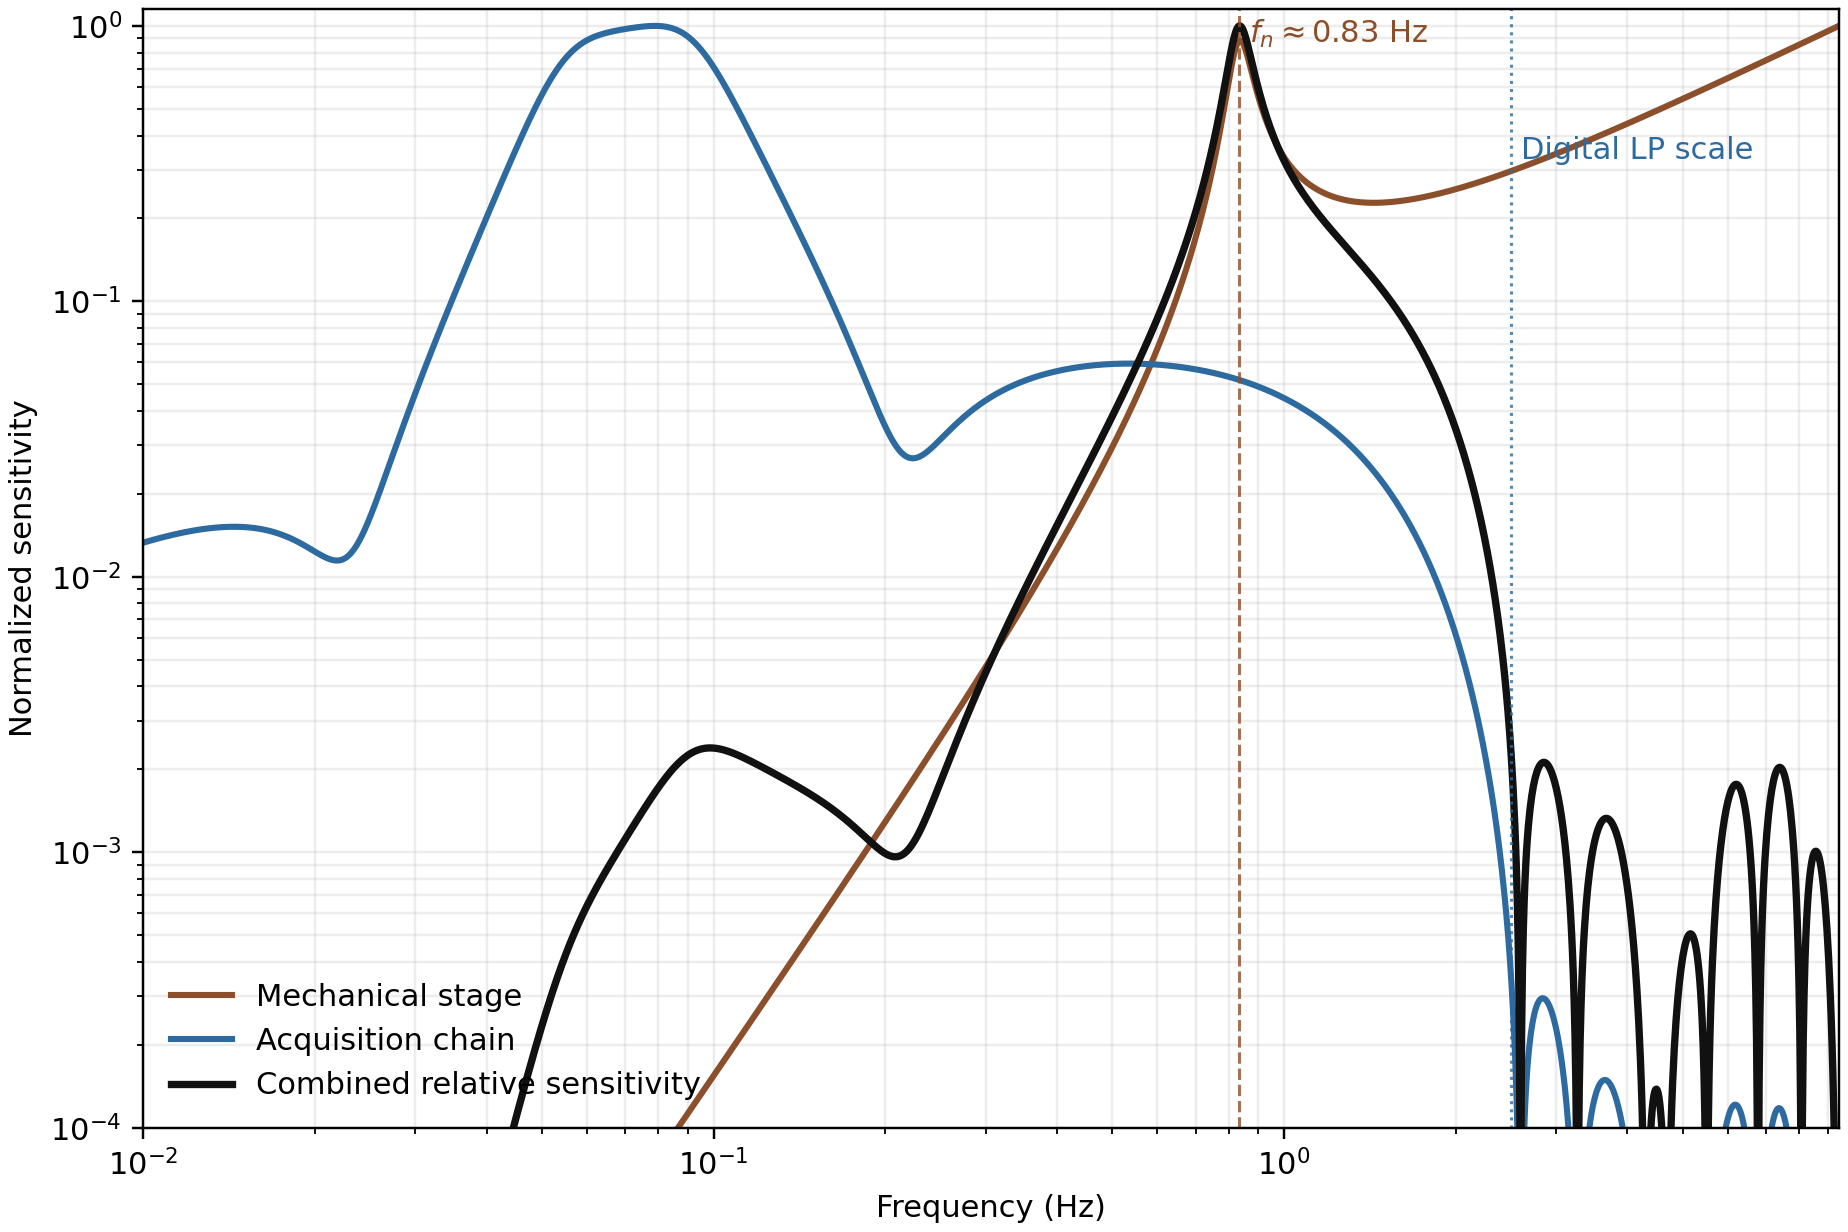
\includegraphics[width=0.84\linewidth]{images/sensitivity_model.png}
  \caption{Predicted relative sensitivity of the seismometer.}
  \label{fig:sensitivity-model}
\end{figure}

Figure~\ref{fig:sensitivity-model} summarizes this model. The combined curve peaks near the mechanical resonance and falls rapidly by a few hertz. This predicts that the instrument should be most responsive to sudden, low-frequency disturbances, while smoother or faster variations should be less visible.

\section{Results and Analysis}
The instrument responded immediately once it had been levelled correctly. If the slinky or magnet was slightly off-center, the baseline became less stable and the signal quality deteriorated. After correction, the oscilloscope showed that table taps produced a clear electrical response, and the amplifier stage increased the visible signal amplitude enough for reliable recording in jAmaSeis.

An additional behavior appeared consistently at startup. When the seismometer was first connected and jAmaSeis began reading, the signal often entered a phase of unusually large oscillation before gradually settling down after about one to two minutes, as shown in Figure~\ref{fig:initializing}. We interpret this as a result of the detrending filter in \texttt{nerdaqII} adjusting to the new baseline.

\begin{figure}[H]
  \centering
  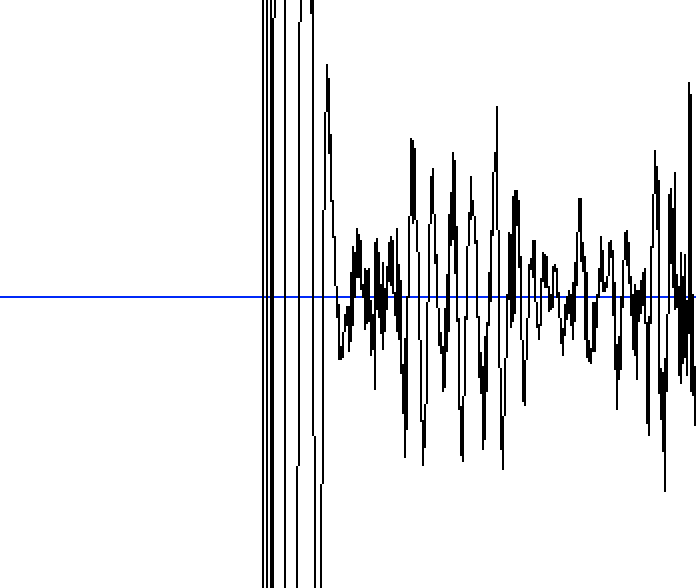
\includegraphics[width=0.58\linewidth]{images/initializing.png}
  \caption{Startup behavior of the seismometer.}
  \label{fig:initializing}
\end{figure}

\subsection{Bridge Test}
The strongest evidence that the instrument worked came from the controlled bridge measurements. Figure~\ref{fig:trace-comparison} shows an \SI{80}{\second} window around the largest transient in a bridge run and, for comparison, an equally sized window from the bus-loop dataset. In the bridge data, the response was sharp and isolated, which is consistent with a nearby impulsive source such as a jump. For the bridge window shown, the recorded signal had a peak-to-peak variation of about 5638 ADC counts and an RMS amplitude of about 645 counts. These large excursions were easy to distinguish from the quieter background trace.

During the same bridge session, we found that walking quietly across the bridge did not produce a significant signal above the background, whereas running and especially jumping generated clear transients. We also noticed that the amplitude changed more strongly when the impact point moved closer to or farther from the end of the bridge than when it moved by a similar amount relative to the instrument itself. Because the seismometer was fixed near the bridge midpoint, this suggests that the bridge behaved as a coupled vibrating structure and that the response depended strongly on how the impact excited the bridge's low-order modes relative to the supports, not simply on the local distance between the jumper and the instrument.

This behavior agrees well with the theory in Figure~\ref{fig:sensitivity-model}. Quiet walking loads the bridge more gradually and therefore contributes less energy in the low frequency band where the instrument is most sensitive. Running and jumping create sharper forcing and excite the bridge modes more strongly near the seismometer's preferred band, so they produce much clearer signals. The dependence on position along the bridge also supports the view that the bridge and seismometer were responding as a coupled vibrational system rather than as a simple local impact sensor.

\begin{figure}[H]
  \centering
  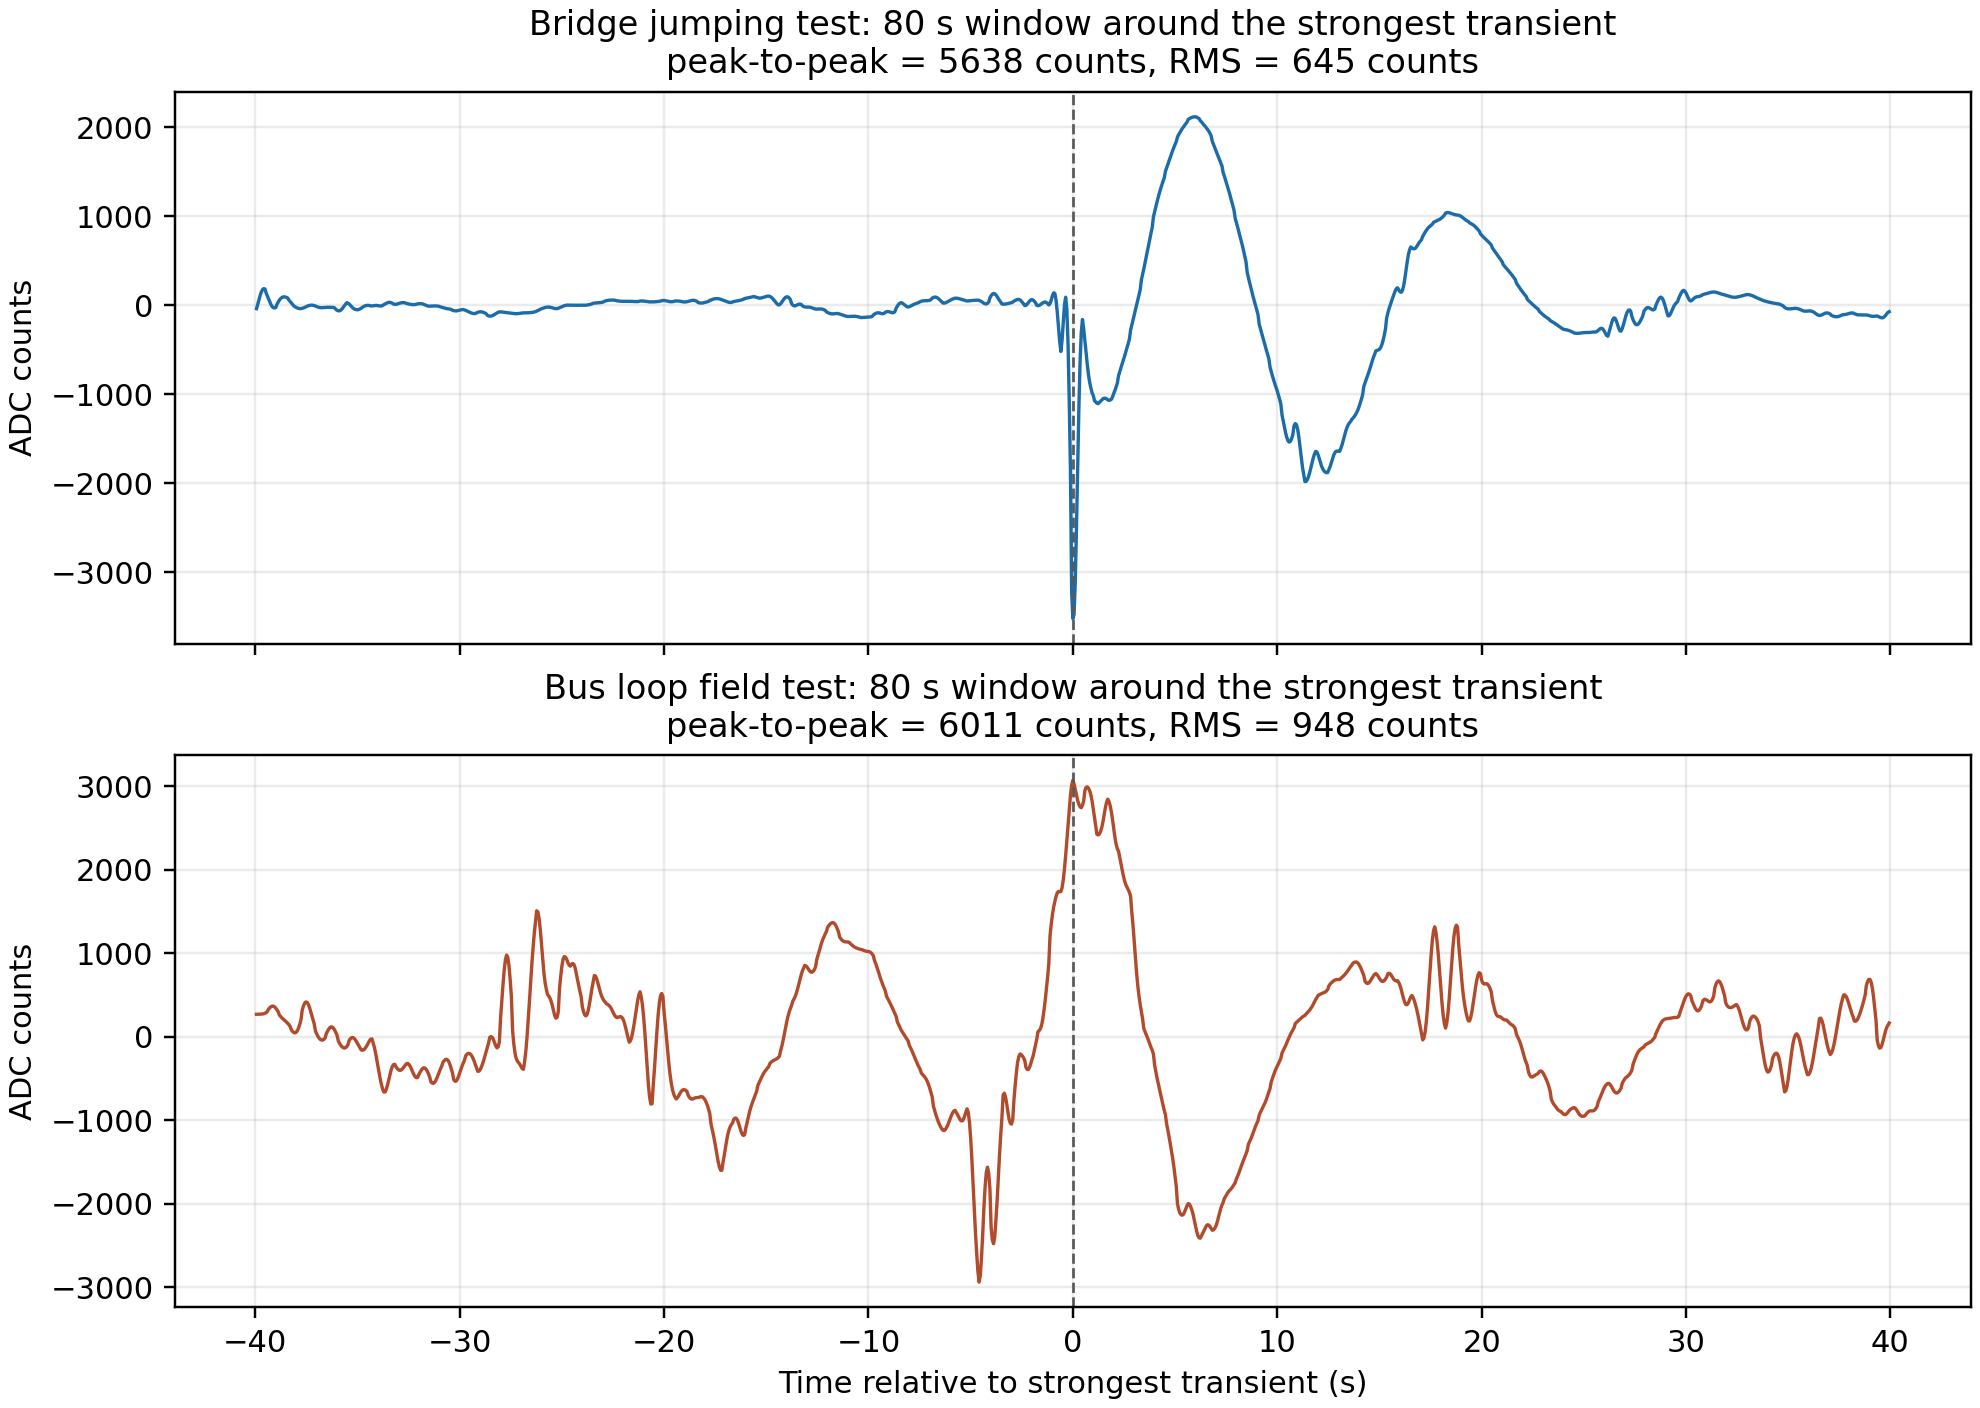
\includegraphics[width=0.92\linewidth]{images/bridge_bus_trace_comparison.png}
  \caption{Comparison of representative traces from the bridge jumping test and the bus loop field test. (A resonance with a period of about 12s is visible.)}
  \label{fig:trace-comparison}
\end{figure}

\subsection{Bus Loop Test}
The bus loop measurements were more difficult to interpret. Figure~\ref{fig:bus-loop-field} shows the annotated outdoor record. We filmed the experiment and then used the video timestamp to label several vehicle passages and nearby footsteps directly on the jAmaSeis screenshot. The outdoor data did contain obvious disturbances, and the largest window we extracted had a peak-to-peak variation of about 6011 ADC counts with an RMS amplitude of about 948 counts. However, it is hard to identify the impact of each source. We suspected that this signal was produced by a person rushing to catch a bus running past the seismometer which explain the gradually increasing and then decreasing amplitude (see Figure~\ref{fig:bus-loop-field}). Unlike the bridge test, where the disturbance time was controlled, the bus-loop record may also include other possible contributors such as wind, curb impacts, nearby traffic, and vibrations transmitted through the pavement and building structure. For that reason, the outdoor result was best treated as suggestive rather than definitive.

\begin{figure}[H]
  \centering
  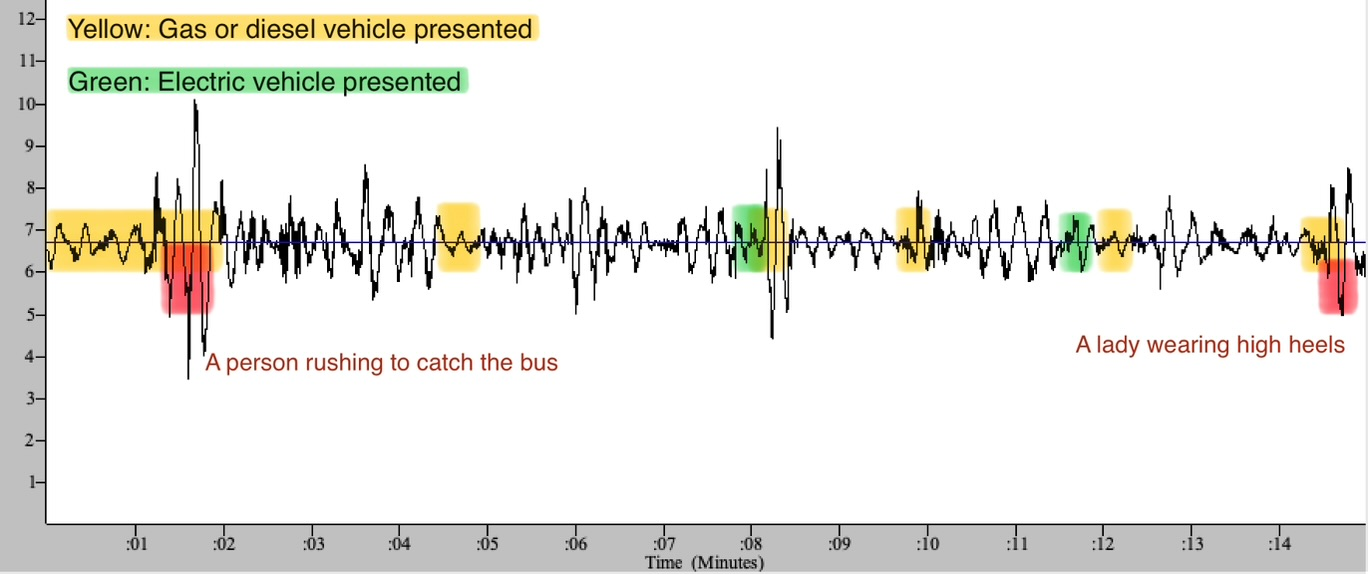
\includegraphics[width=\linewidth]{images/bus_loop.jpeg}
  \caption{Annotated jAmaSeis display from the real-world measurement near the campus bus loop.}
  \label{fig:bus-loop-field}
\end{figure}

% To look for a characteristic signature in the outdoor data, we also examined the frequency-domain view saved during the bus-loop test. As shown in Figure~\ref{fig:bus-spectrum}, the spectrum did not exhibit a single narrow feature that could be assigned unambiguously to bus traffic. Instead, the disturbance energy was spread over a broad low-frequency range. This behavior is consistent with a mixture of environmental vibrations and with the fact that the mechanical instrument itself has a finite resonance width rather than responding equally to every frequency. 

The video-based annotations suggest a qualitative difference between vehicle types: both electric vehicles and gas/diesel vehicles produced disturbances associated with the motion of a heavy vehicle across the pavement, but the gas/diesel passages more often coincided with longer and less impulsive oscillatory intervals, while electric vehicles tended to resemble shorter movement-dominated disturbances. This is only a qualitative trend in our data, but it suggests that engine vibration may add to the seismic signature beyond the effect of vehicle passage alone.

The theory also helps explain why the bus loop result was less clean than the bridge result. The seismometer is most sensitive to low frequency impulsive motion, so nearby footsteps and high heels can compete strongly with vehicle signals even though the vehicles are larger sources overall. A bus passing at some distance may spread its forcing over time and over multiple structural paths, which makes it harder to isolate than a direct, sharp bridge impact. The broad band spectrum is therefore consistent with several overlapping sources passing through an instrument that is selective but not source-specific.

% \begin{figure}[H]
%   \centering
%   \begin{subfigure}[t]{0.48\linewidth}
%     \centering
%     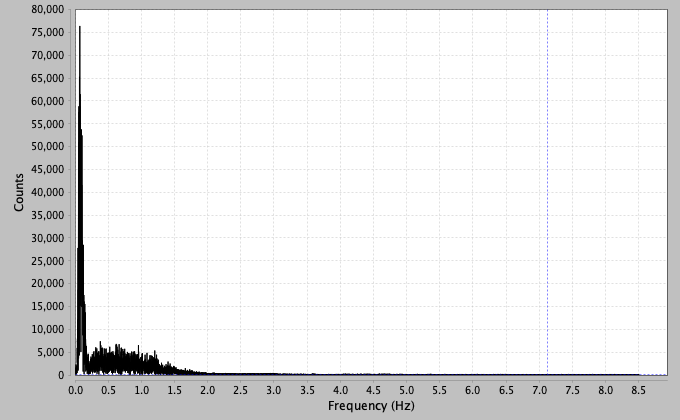
\includegraphics[width=\linewidth]{images/bus_loop_frequency.png}
%     \caption{Frequency-domain view.}
%   \end{subfigure}
%   \hfill
%   \begin{subfigure}[t]{0.48\linewidth}
%     \centering
%     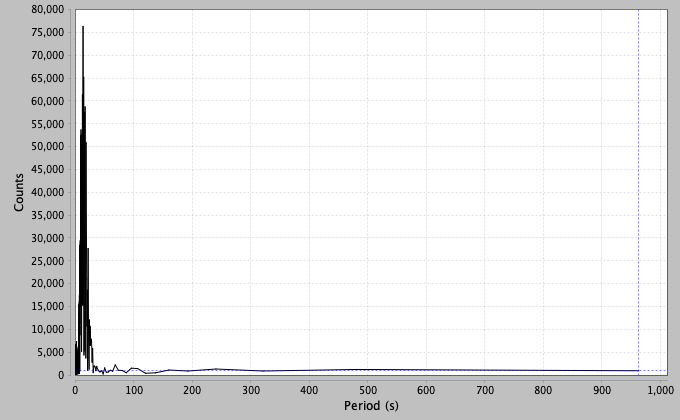
\includegraphics[width=\linewidth]{images/bus_loop_period.png}
%     \caption{Period-domain view.}
%   \end{subfigure}
%   \caption{Saved spectral views from the bus-loop test. The response is broad-band rather than dominated by one clear feature.}
%   \label{fig:bus-spectrum}
% \end{figure}

\subsection{Frequency Domain Analysis}
To compare the measured signals with the theoretical sensitivity model more directly, we computed FFTs of the bridge and bus loop traces. Figure~\ref{fig:fft-vs-model} shows the FFT of the same \SI{80}{\second} windows used in the time domain comparison, overlaid with both the acquisition-chain model and the full combined sensitivity model. In both the bridge and bus loop windows, the dominant low frequency peak lies close to the long period maximum of the acquisition chain rather than to the mechanical resonance near \SI{0.83}{\hertz}. This indicates that when a long window around the strongest transient is examined as a whole, the displayed spectrum is shaped mainly by the default \texttt{nerdaqII} filtering, especially its low frequency emphasis around periods of roughly 10--13 s.

\begin{figure}[H]
  \centering
  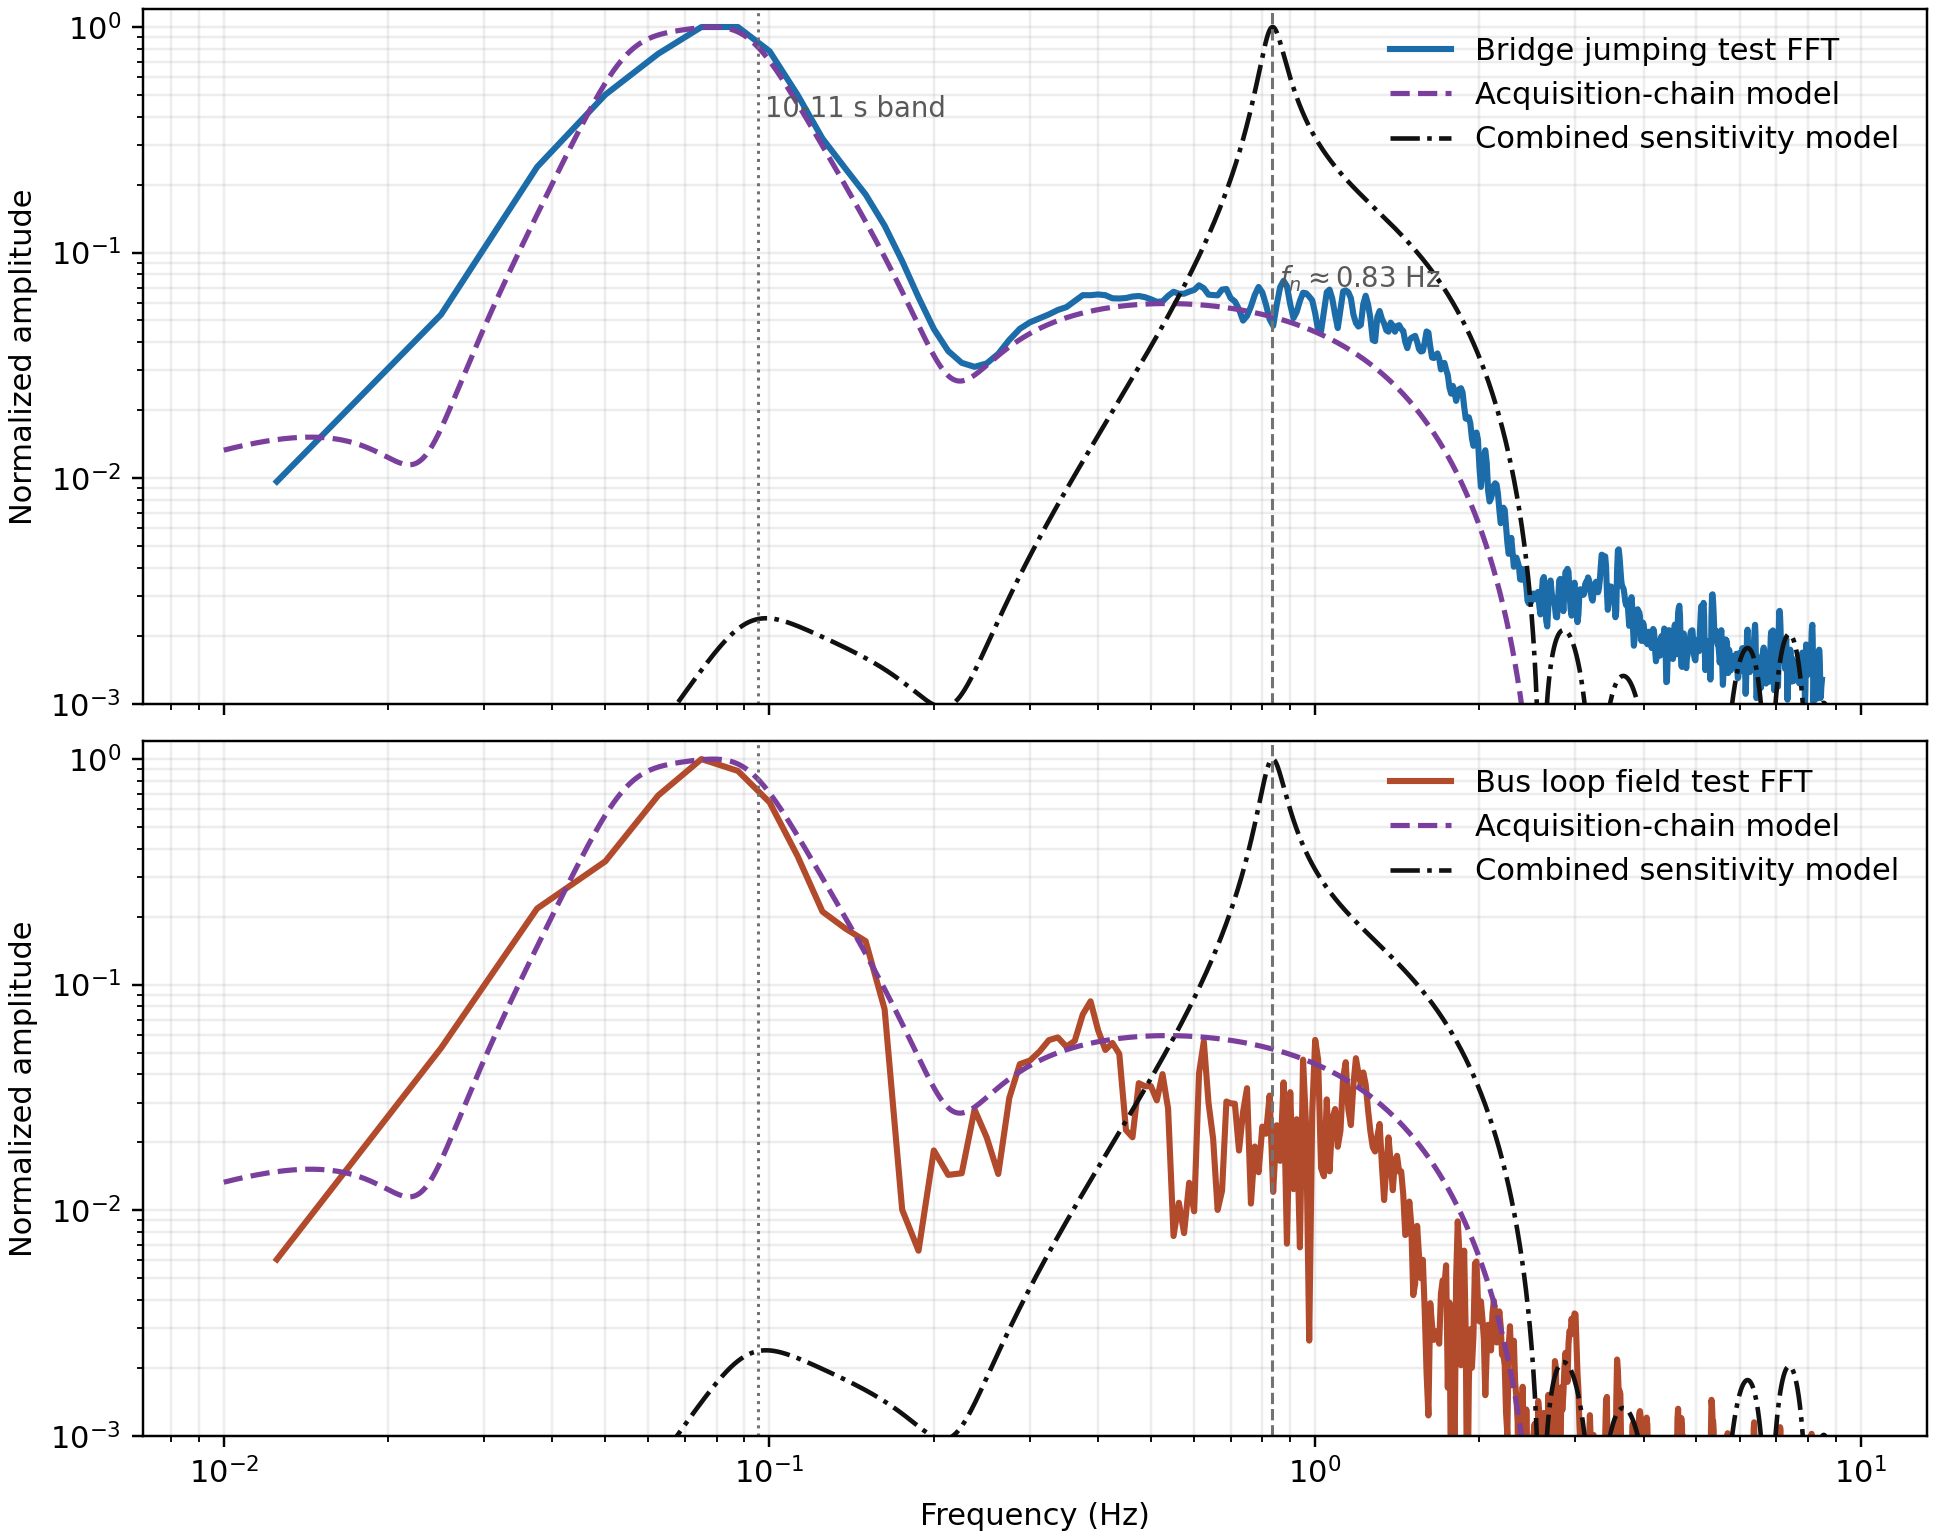
\includegraphics[width=0.88\linewidth]{images/fft_vs_sensitivity_model.png}
  \caption{FFT of the \SI{80}{\second} bridge and bus loop windows compared with the modeled acquisition chain response and the full sensitivity model.}
  \label{fig:fft-vs-model}
\end{figure}

The bridge test allows a more controlled separation between background and post-impact ringing. Figure~\ref{fig:bridge-segment-fft} compares the FFT of a pre-event background segment with the FFT of the post-event ringing segment only. The background spectrum reproduces the acquisition-chain preference quite closely, while the post-event ringing shows an additional visible resonance near the natural frequency of the spring mass system. This is an important result: the instrument output contains both the digital filter signature and the physical bridge/seismometer response, but they appear most clearly in different parts of the record. The long period background and full window spectra are dominated by the acquisition chain, whereas the post-impact ringing reveals the mechanical resonance more clearly.

\begin{figure}[H]
  \centering
  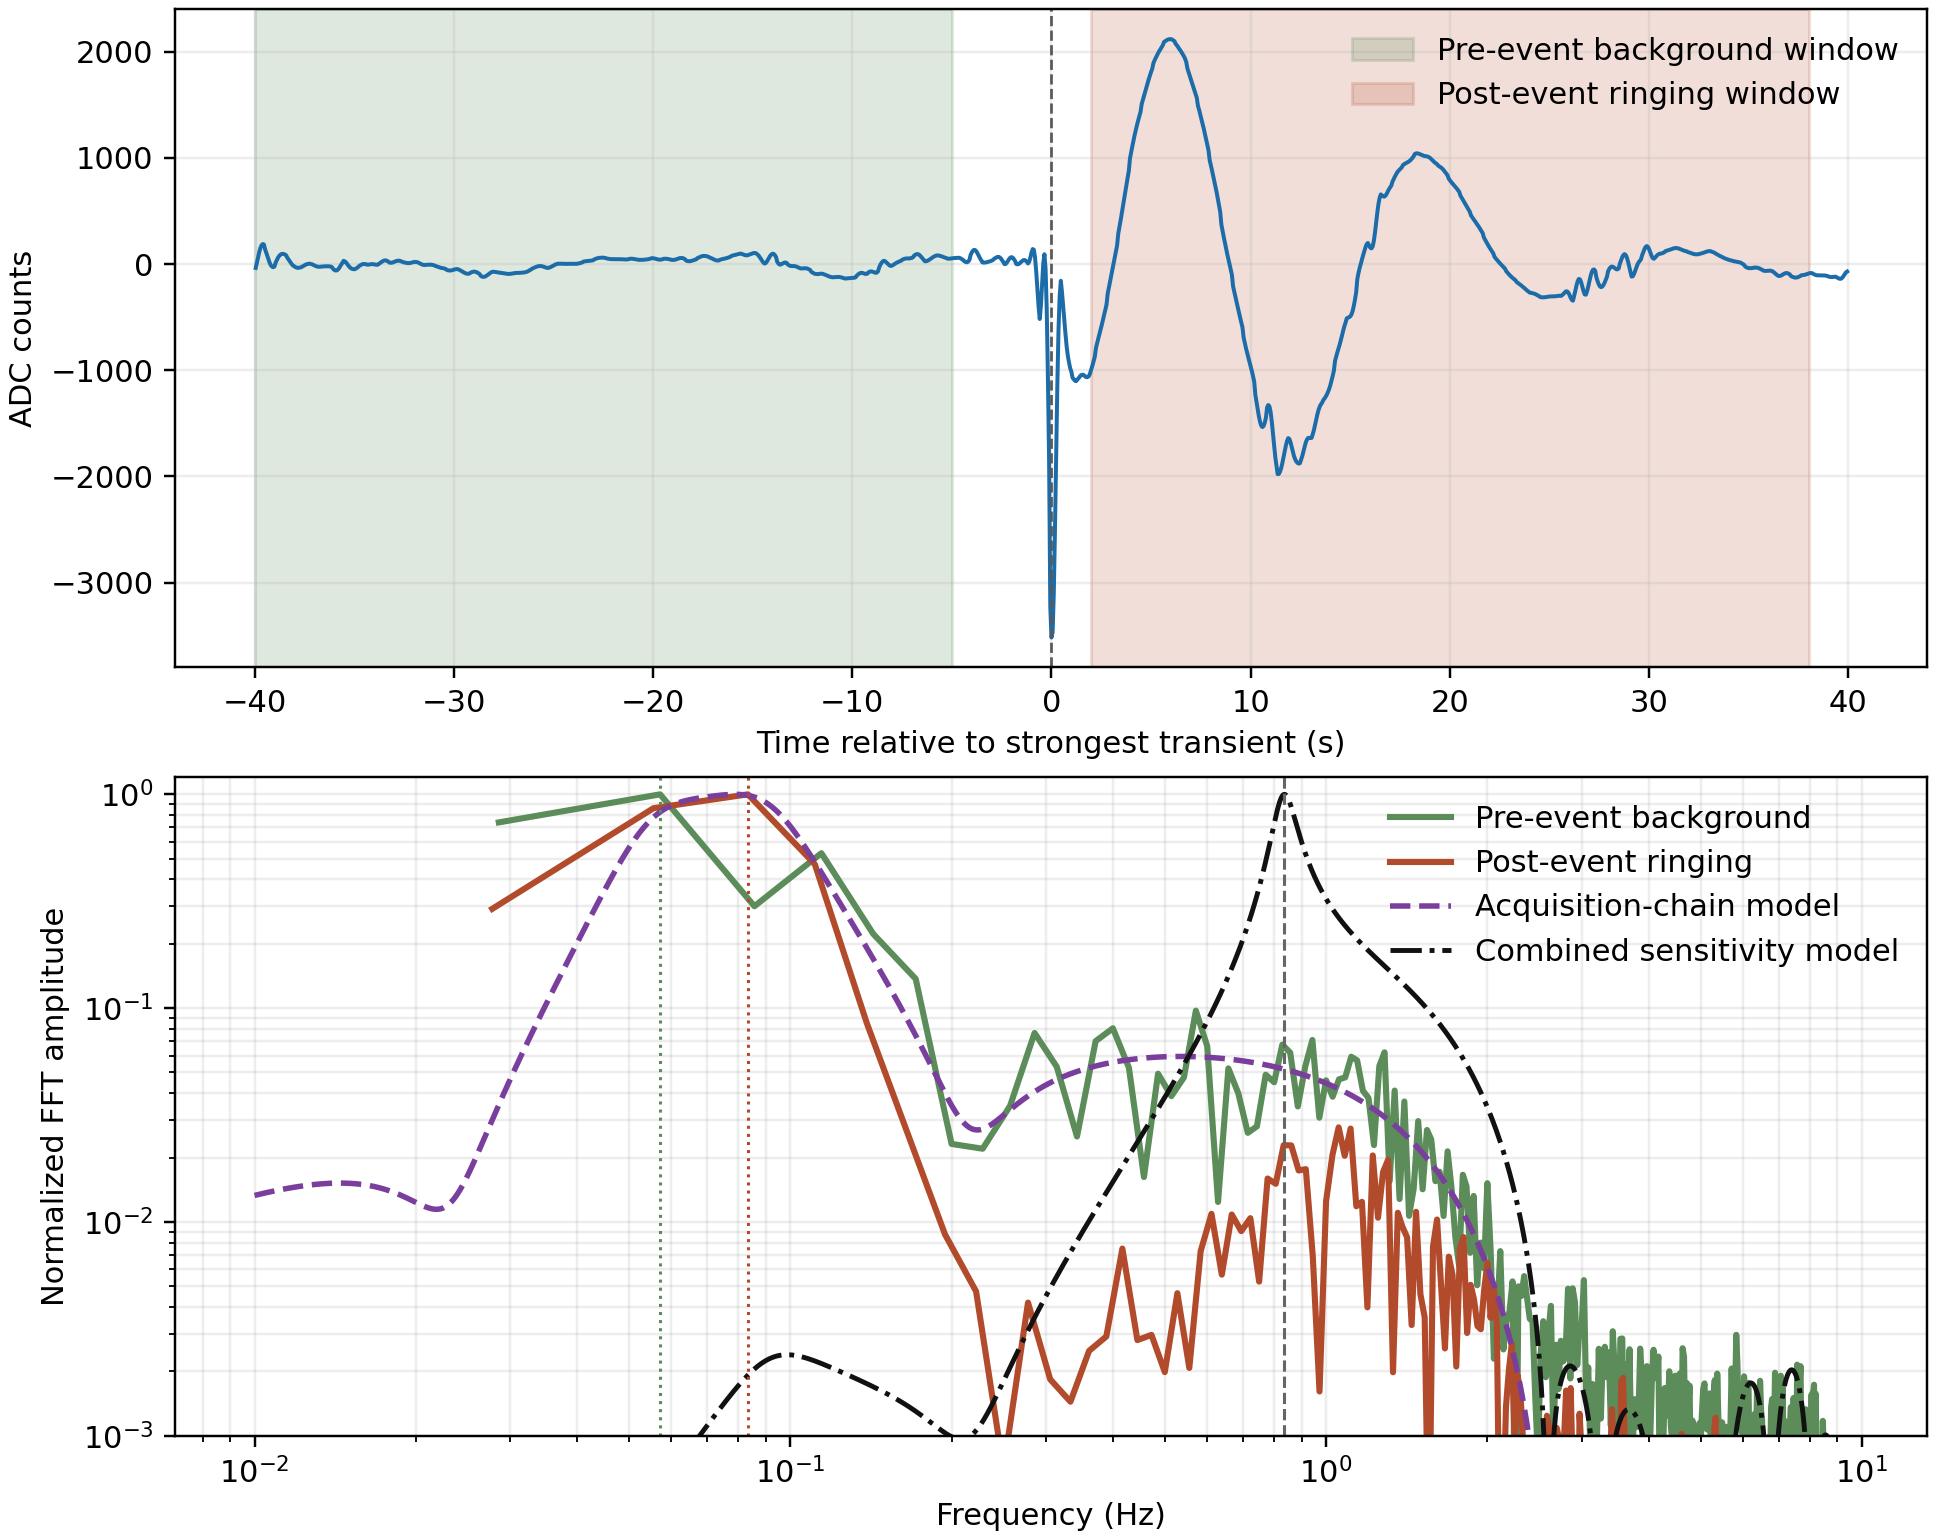
\includegraphics[width=0.88\linewidth]{images/bridge_segment_fft.png}
  \caption{FFT of the pre-event background noise and the post-event ringing in the bridge test compared with the sensitivity model.}
  \label{fig:bridge-segment-fft}
\end{figure}

\section{Discussion}
The project showed that the combined mechanical and digital response is quite narrow compared with a broadband vibration sensor. For the intended purpose of detecting earthquakes, this is useful because it suppresses much of the irrelevant high-frequency noise and makes low frequency vibrations and impulses easier to see. However, that narrow spectrum also distorts the frequency characteristics of other sources if the instrument is repurposed. In the bus loop measurement, for example, the recorded signal reflects the response of the acquisition chain at least as much as it reflects the original source spectrum, so frequency based source identification becomes difficult without additional calibration or raw data.

The comparison between the FFT data and the model supports this interpretation. The acquisition chain model matches the background noise and the full \SI{80}{\second} spectra quite well, which suggests that the digital processing is being captured reasonably by the model. 

It is important to note that we are assuming that the mechanical input to the harmonic oscillator is of equal displacement amplitude at each frequency. However, the actual input could also be of equal velocity or equal acceleration amplitude, which would change the predicted sensitivity curve. In contrast to the high confidence in the acquisition chain model, distinguishing between the three assumptions requires more controlled data than we collected here.

If the experiment were repeated, the best improvements would be targeted rather than generic. The spring constant could be tuned so that the mechanical resonance better matches the frequency of the target source. The analog filter and amplifier could then be adjusted so that the system gives more gain in that same band while rejecting irrelevant noise. For example, if the goal were to distinguish diesel or gasoline engines from electric vehicles, the spring, analog filter, and digital post-processing should all be tuned around the frequency region where engine vibrations differ most from vehicle passing. It is also possible to calibrate its sensitivity by applying a known vibration to the base and measuring the output, which would allow the raw data to be interpreted in physical units rather than just ADC counts.

\section{Conclusion}
We assembled and tested a slinky based seismometer that converted vibration into an electrical signal and displayed it through an acquisition chain. The instrument clearly detected controlled vibrations in the bridge jumping test, demonstrating that the combined mechanical and electronic system worked. Frequency domain analysis showed that the default acquisition chain strongly shapes the recorded spectrum, especially in long windows and background data, while the bridge post-event ringing still preserved evidence of the spring mass resonance near \SI{0.83}{\hertz}. The bus loop measurement showed that the instrument could record substantial outdoor disturbances, but it also showed that real world source identification was more difficult than simply observing a large waveform. 
% Overall, the project met its main goal of building a working vibration detector while also revealing how calibration, amplification, filtering, noise, and experimental design affect the usefulness of the measurements.

\end{document}
